\documentclass[aspectratio=169]{beamer}
\usepackage[utf8]{inputenc}
\usepackage[T1]{fontenc}
\usepackage{svg}

\title{Open Data: \\ Receive it Yourself}
\date[ISPN ’80]{Datenspuren 2022}
\author[]{Tassilo, 0xA, Marenz (dump@dvb.solutions)}

\usetheme{dvb}

\AtBeginSection[]{
  \begin{frame}
    \begin{tikzpicture}
      \fill[rounded corners,dvbyellow,rotate around={30:(-1,0.5)}] (-20.5,0) rectangle (-0.5,2);
      \fill[rounded corners,dvbyellow,rotate around={30:(-1,0.5)}] (-20.5,3) rectangle (-0.5,5);
      \node (logo) at (-18,2) {
        \textbf{ \LARGE \textbf{ \myfont \secname } }
      };
  \end{tikzpicture}
  \end{frame}
}

\newcommand*{\myfont}{\fontfamily{pag}\selectfont}

\begin{document}

\begin{frame}\titlepage
\end{frame}
  
\begin{frame} 
 %\includesvg{dvbdump}
\frametitle{Roadmap} 
%\framesubtitle{The proof uses \textit{reductio ad absurdum}.} 

\begin{enumerate}
    \item VDV 420 explaining the standard
    \item what we are trying to achieve
    \item we had a plan until we saw raw data
    \item We need you !
\end{enumerate}

\end{frame}

\section{Radio \& VDV 420}

\begin{frame}
\frametitle{Receiving data}
\centering
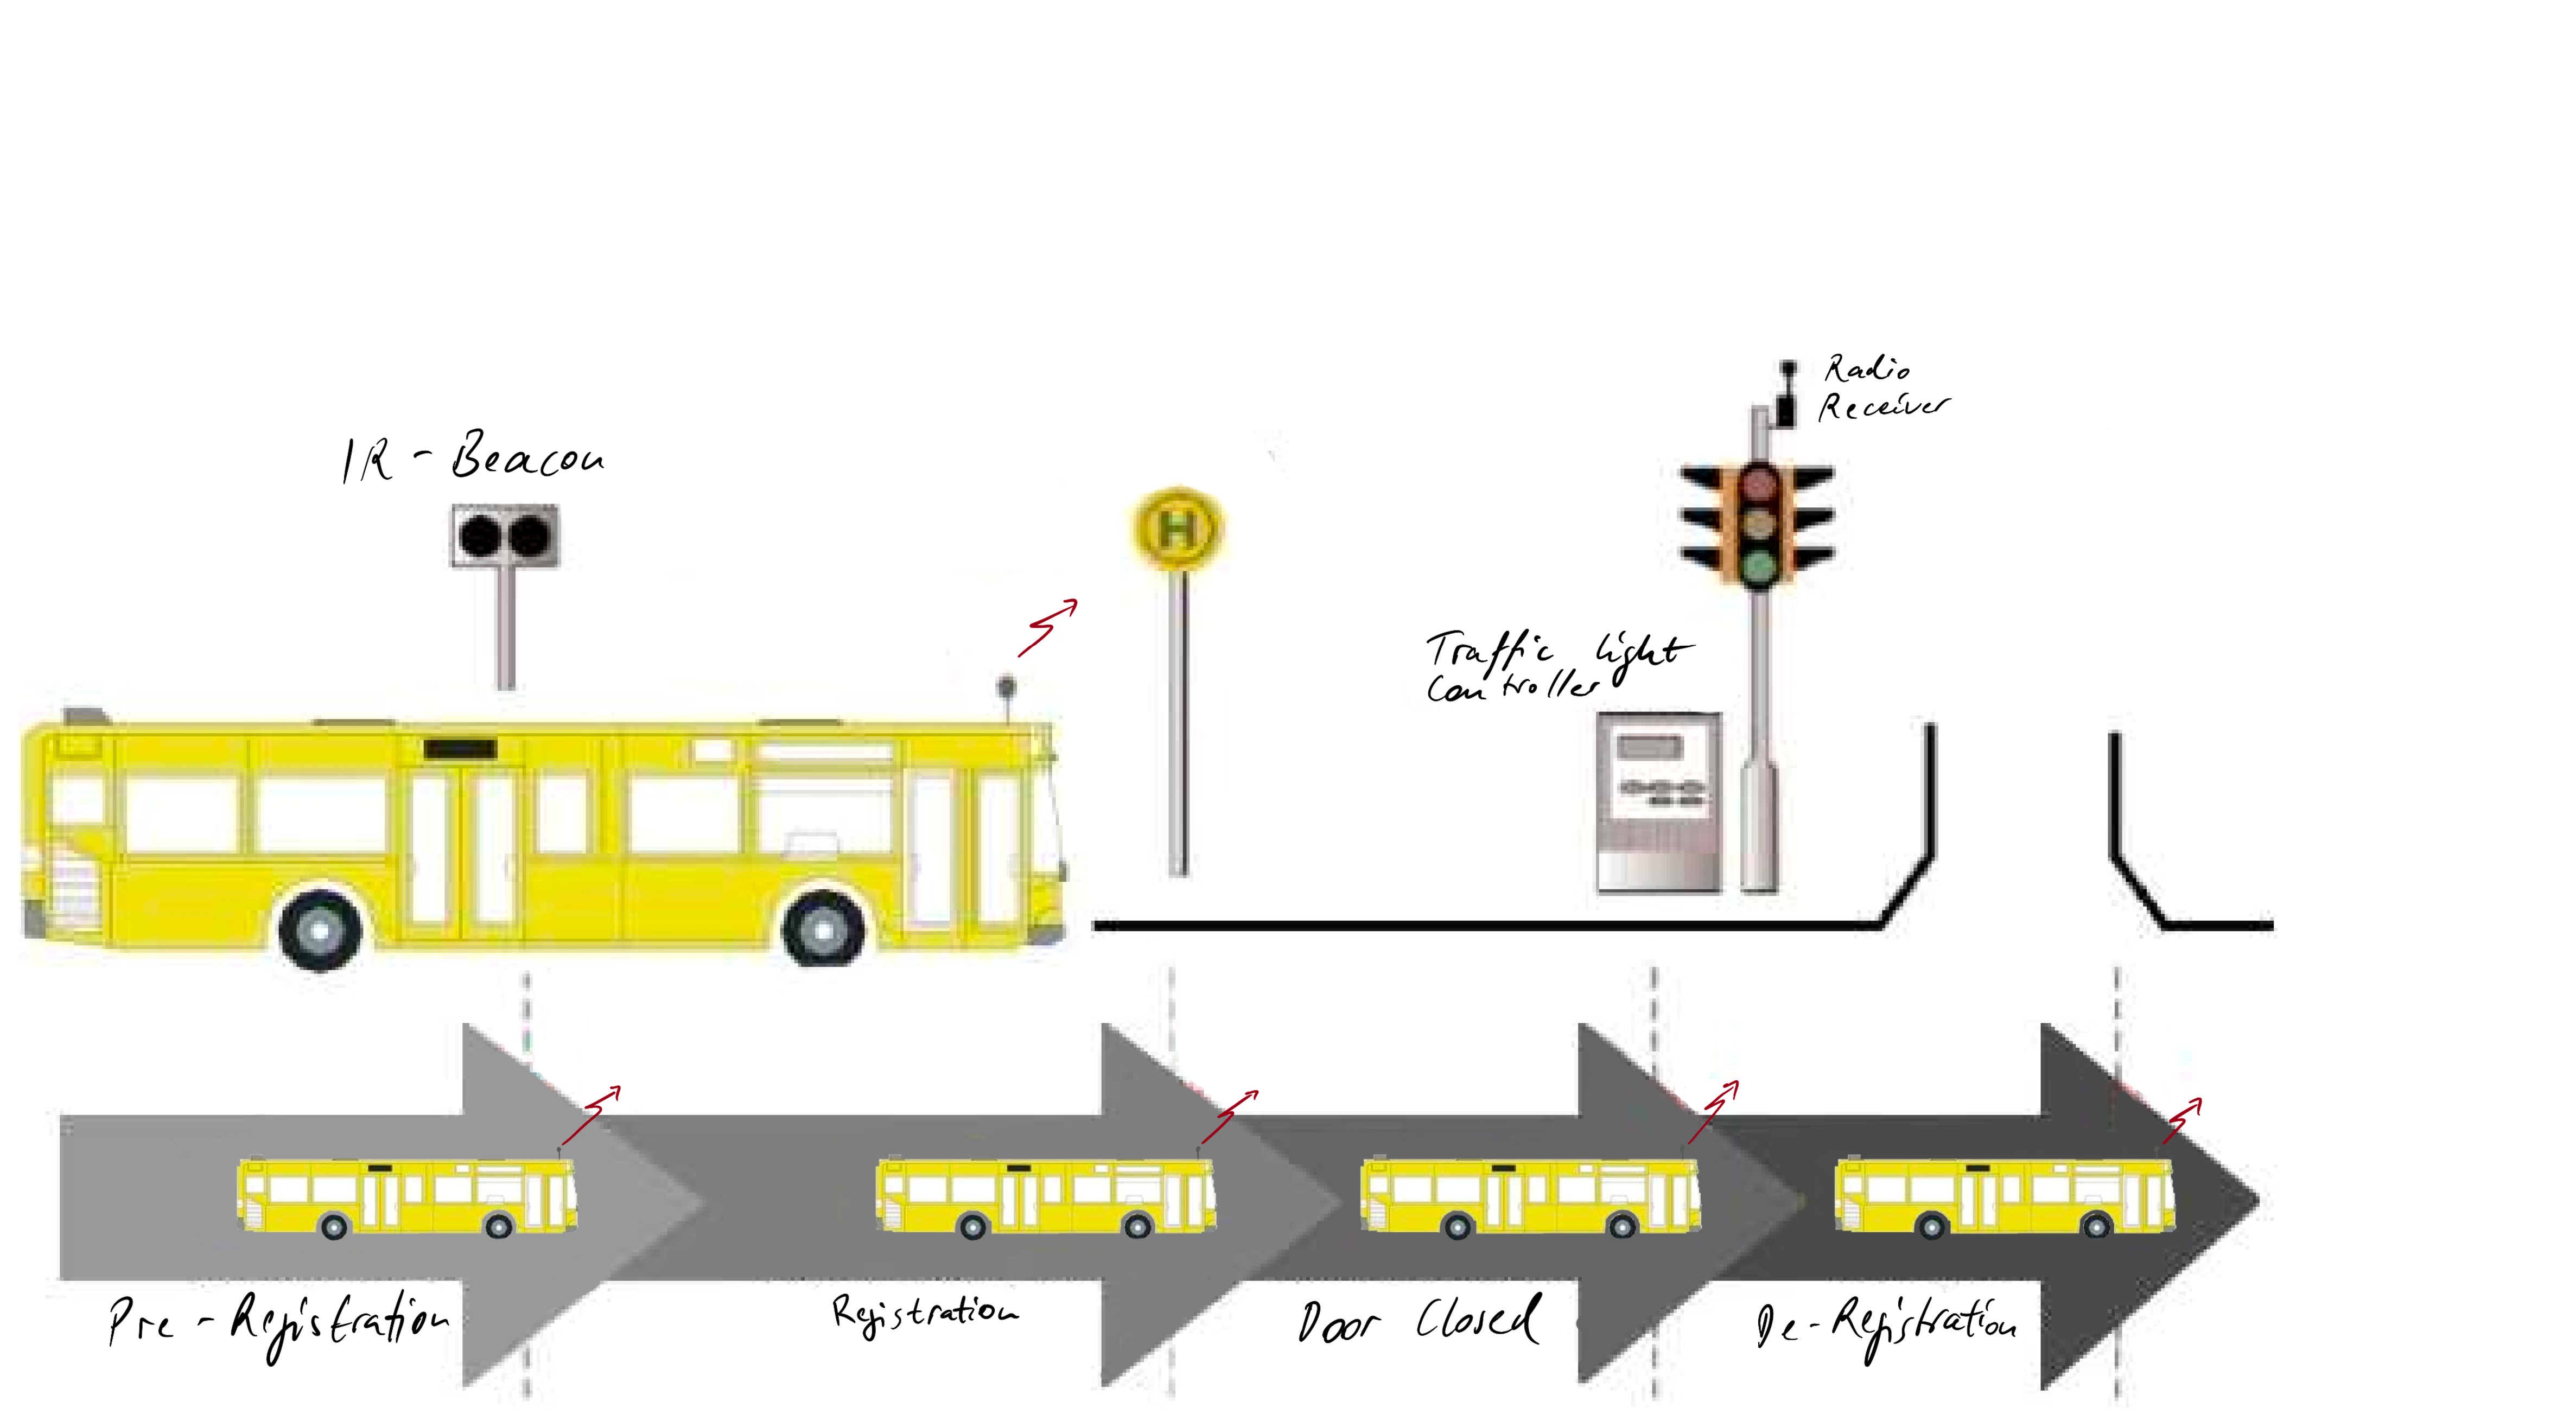
\includegraphics[width=0.8\textwidth]{figs/lsa-beeinflussungs-stecke.pdf}
\end{frame}

\begin{frame}
\frametitle{Receiving data}
\centering
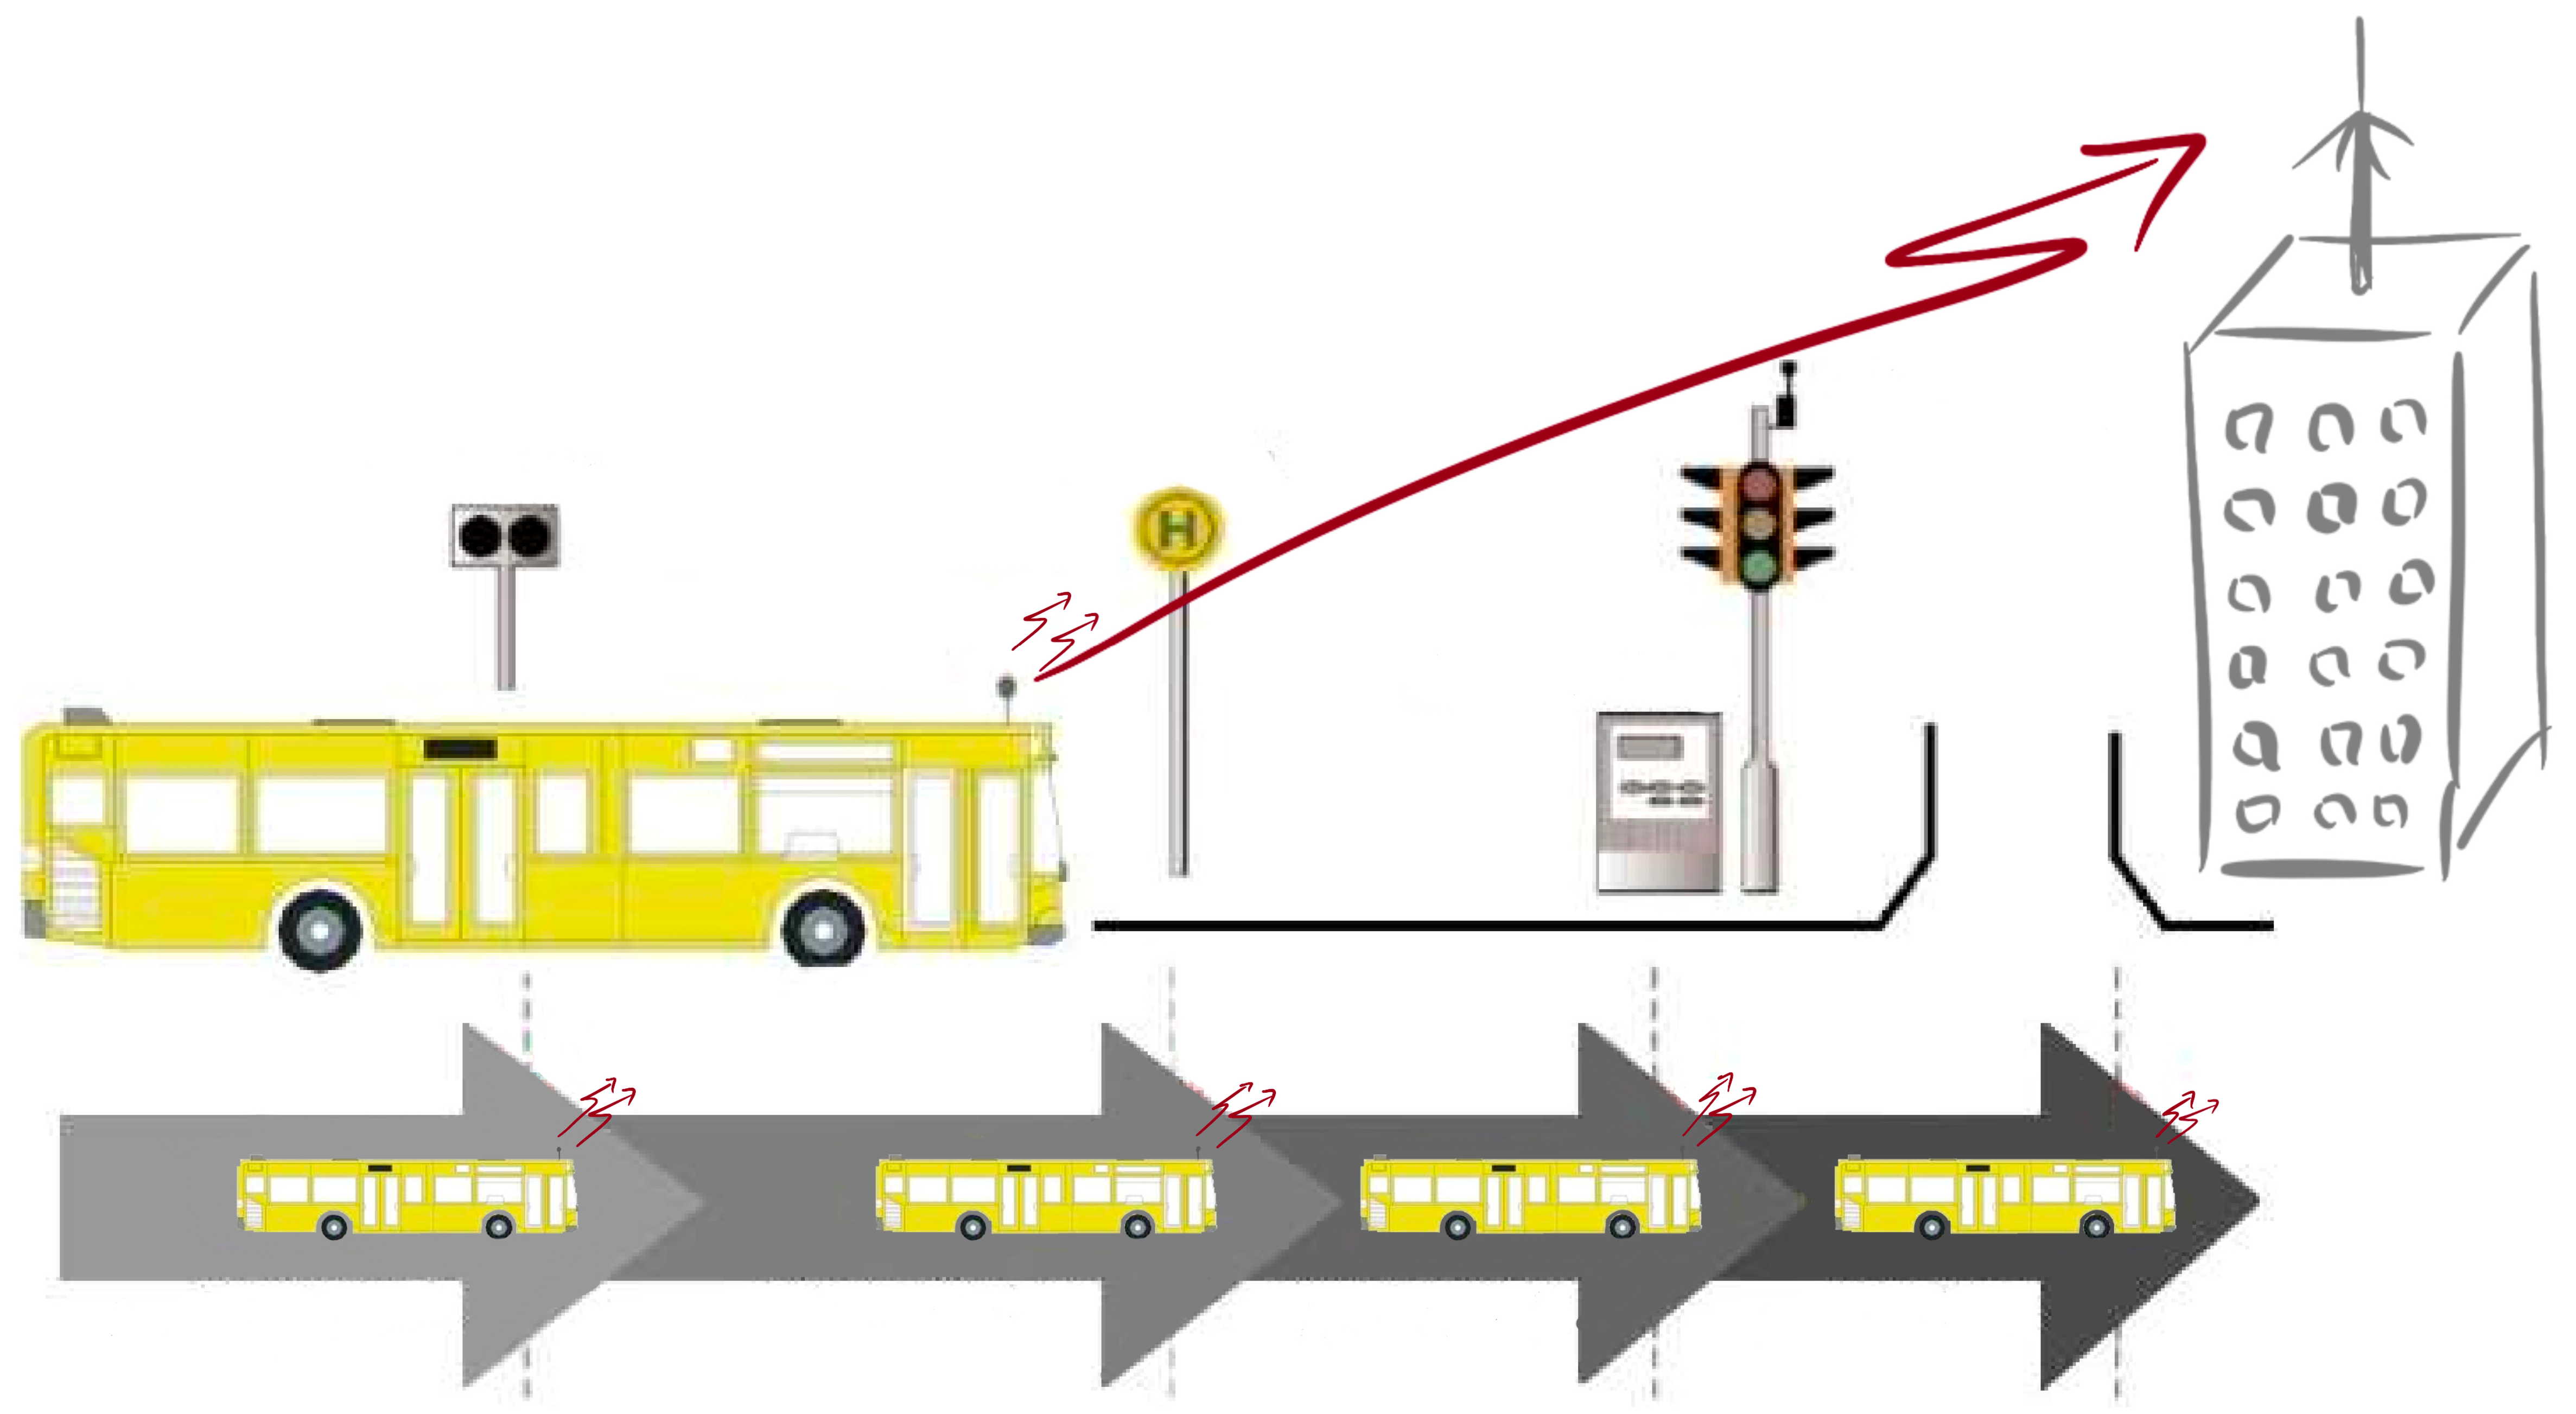
\includegraphics[width=0.8\textwidth]{figs/lsa-beeinflussungs-stecke-mit-antenne.pdf}
\end{frame}

\begin{frame}
\frametitle{Receiving data}
\centering
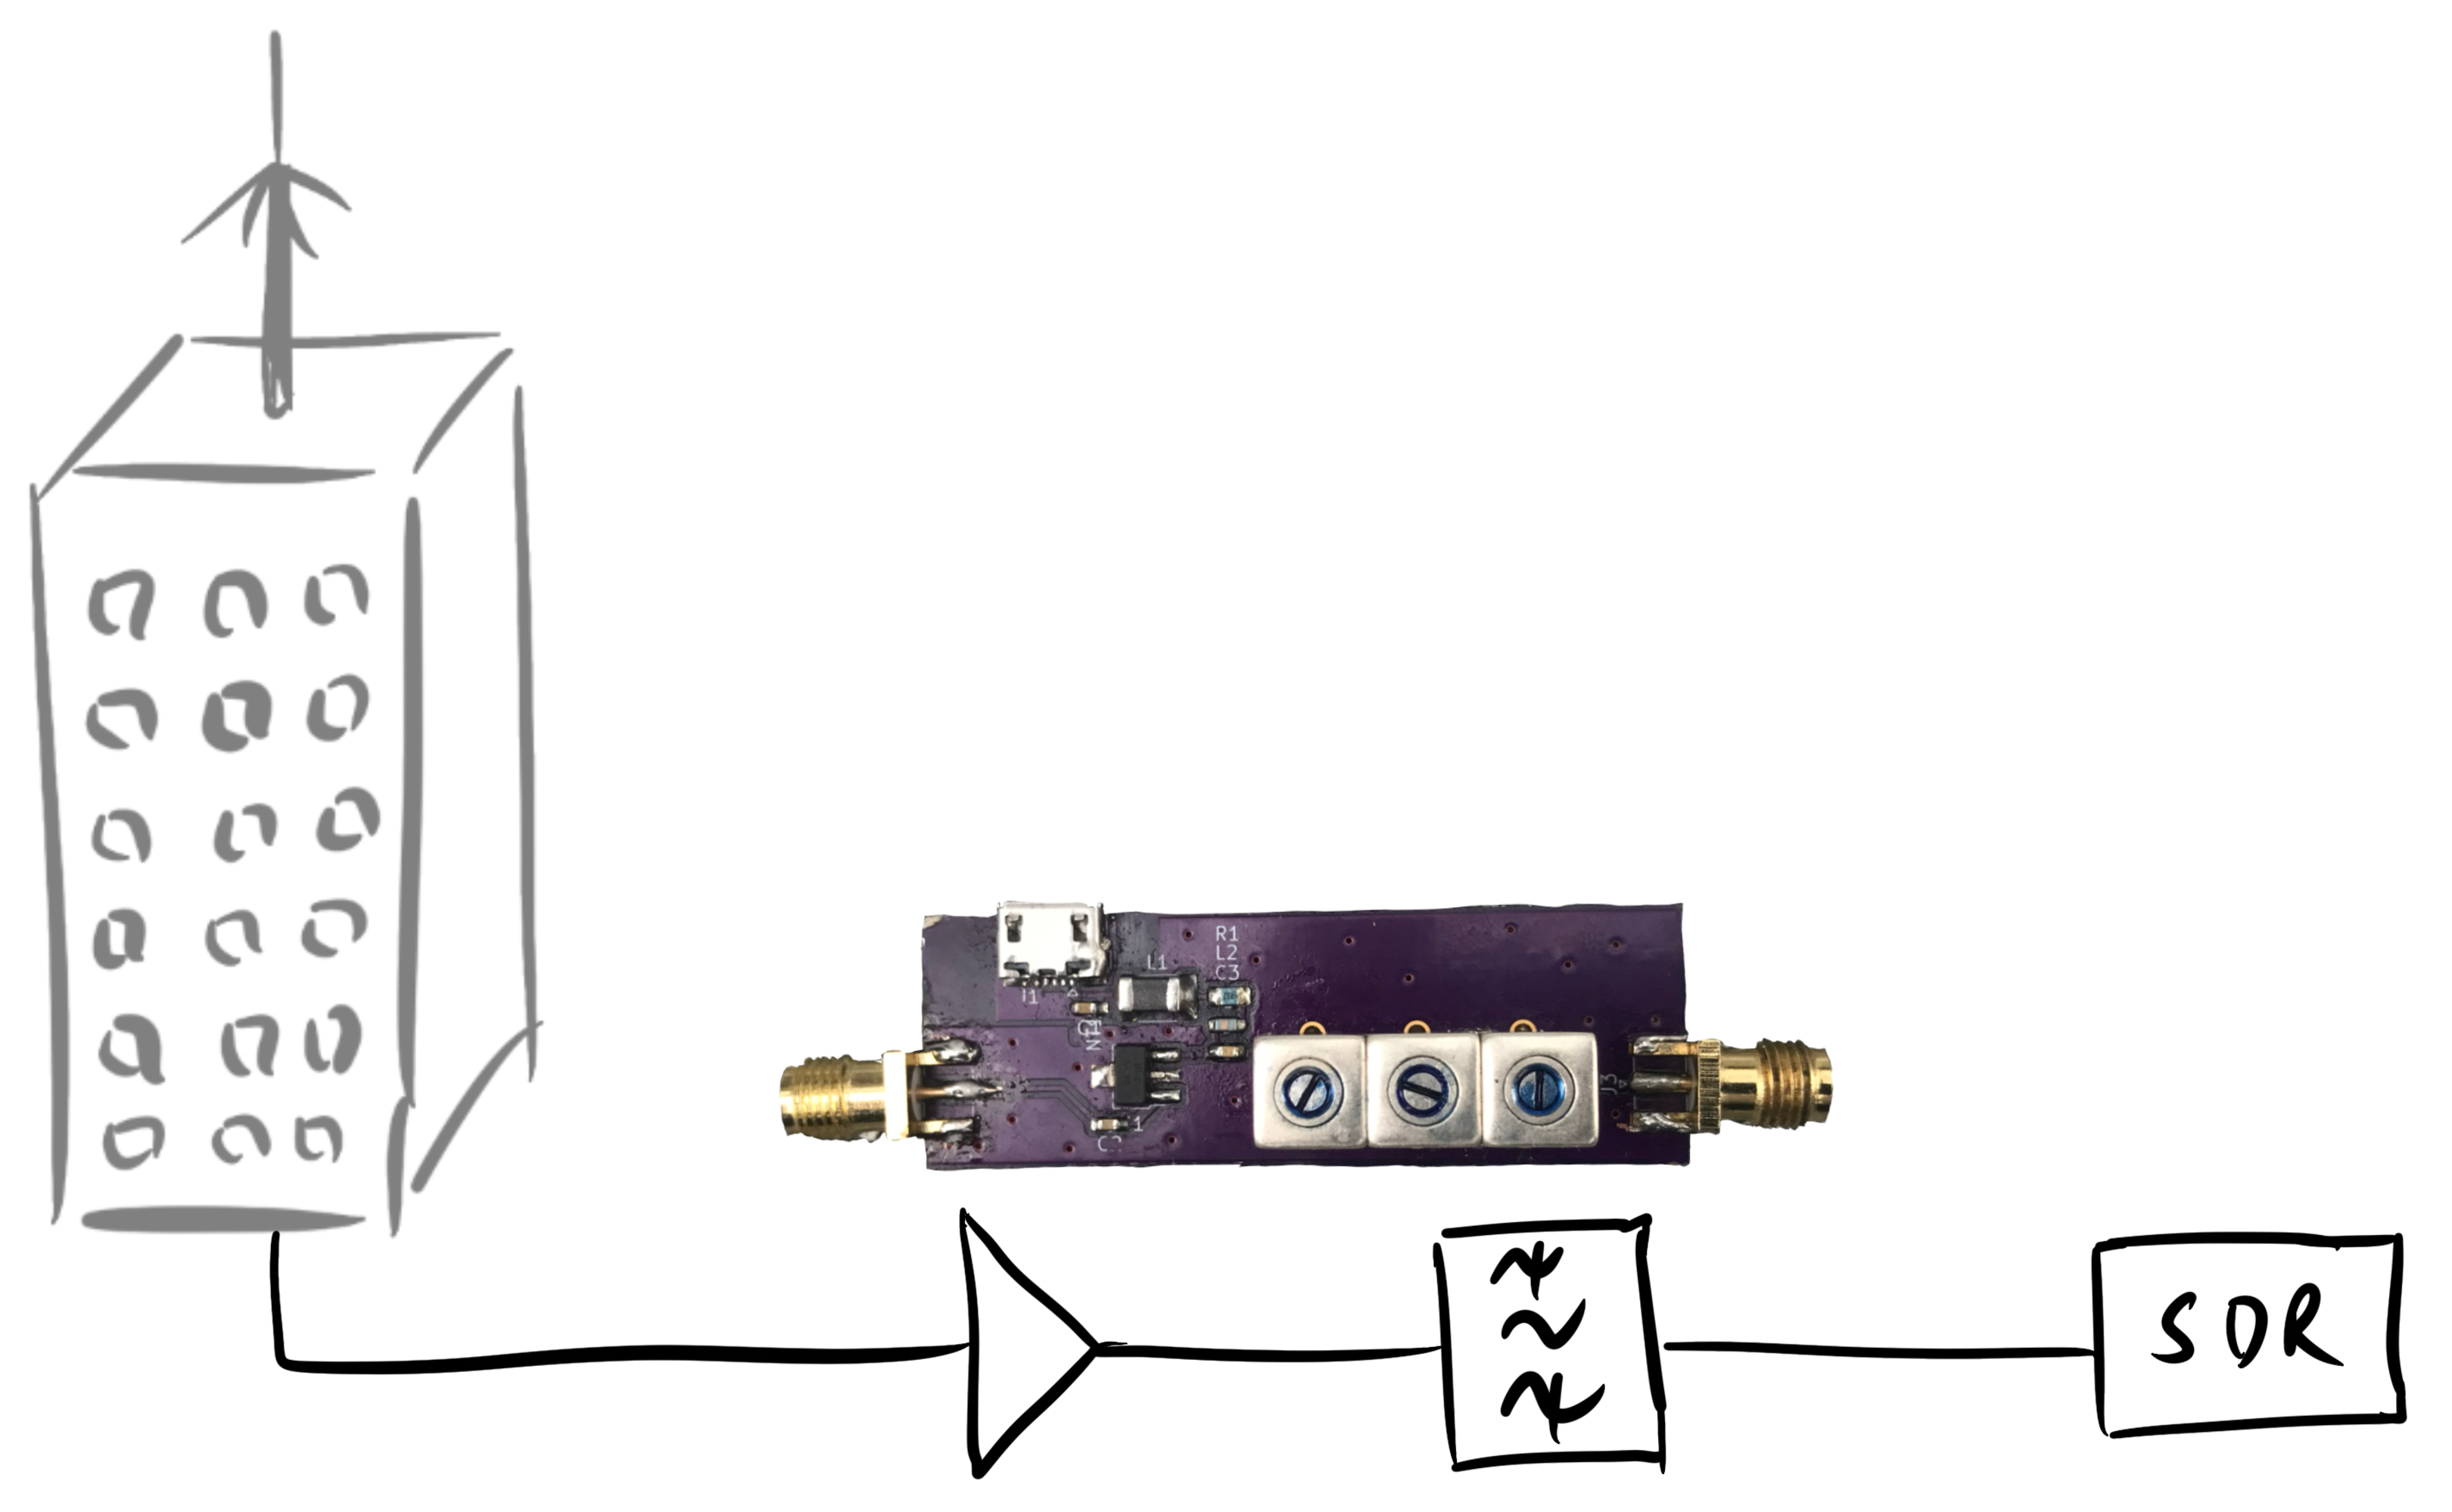
\includegraphics[width=0.7\textwidth]{figs/antenna-filter.pdf}
\end{frame}

\begin{frame}
	\begin{itemize}
	\item telegrams of trams and busses standardized in \href{https://knowhow.vdv.de/documents/420/}{VDV 420}
	\item R09.16 telegramsx used in Dresden
	\end{itemize}
\end{frame}

\begin{frame}
\frametitle{Receiving data}
\centering
% https://opus4.hbz-nrw.de/opus45-bast/frontdoor/deliver/index/docId/2595/file/V353+BF+Gesamtversion.pdf
% page 25

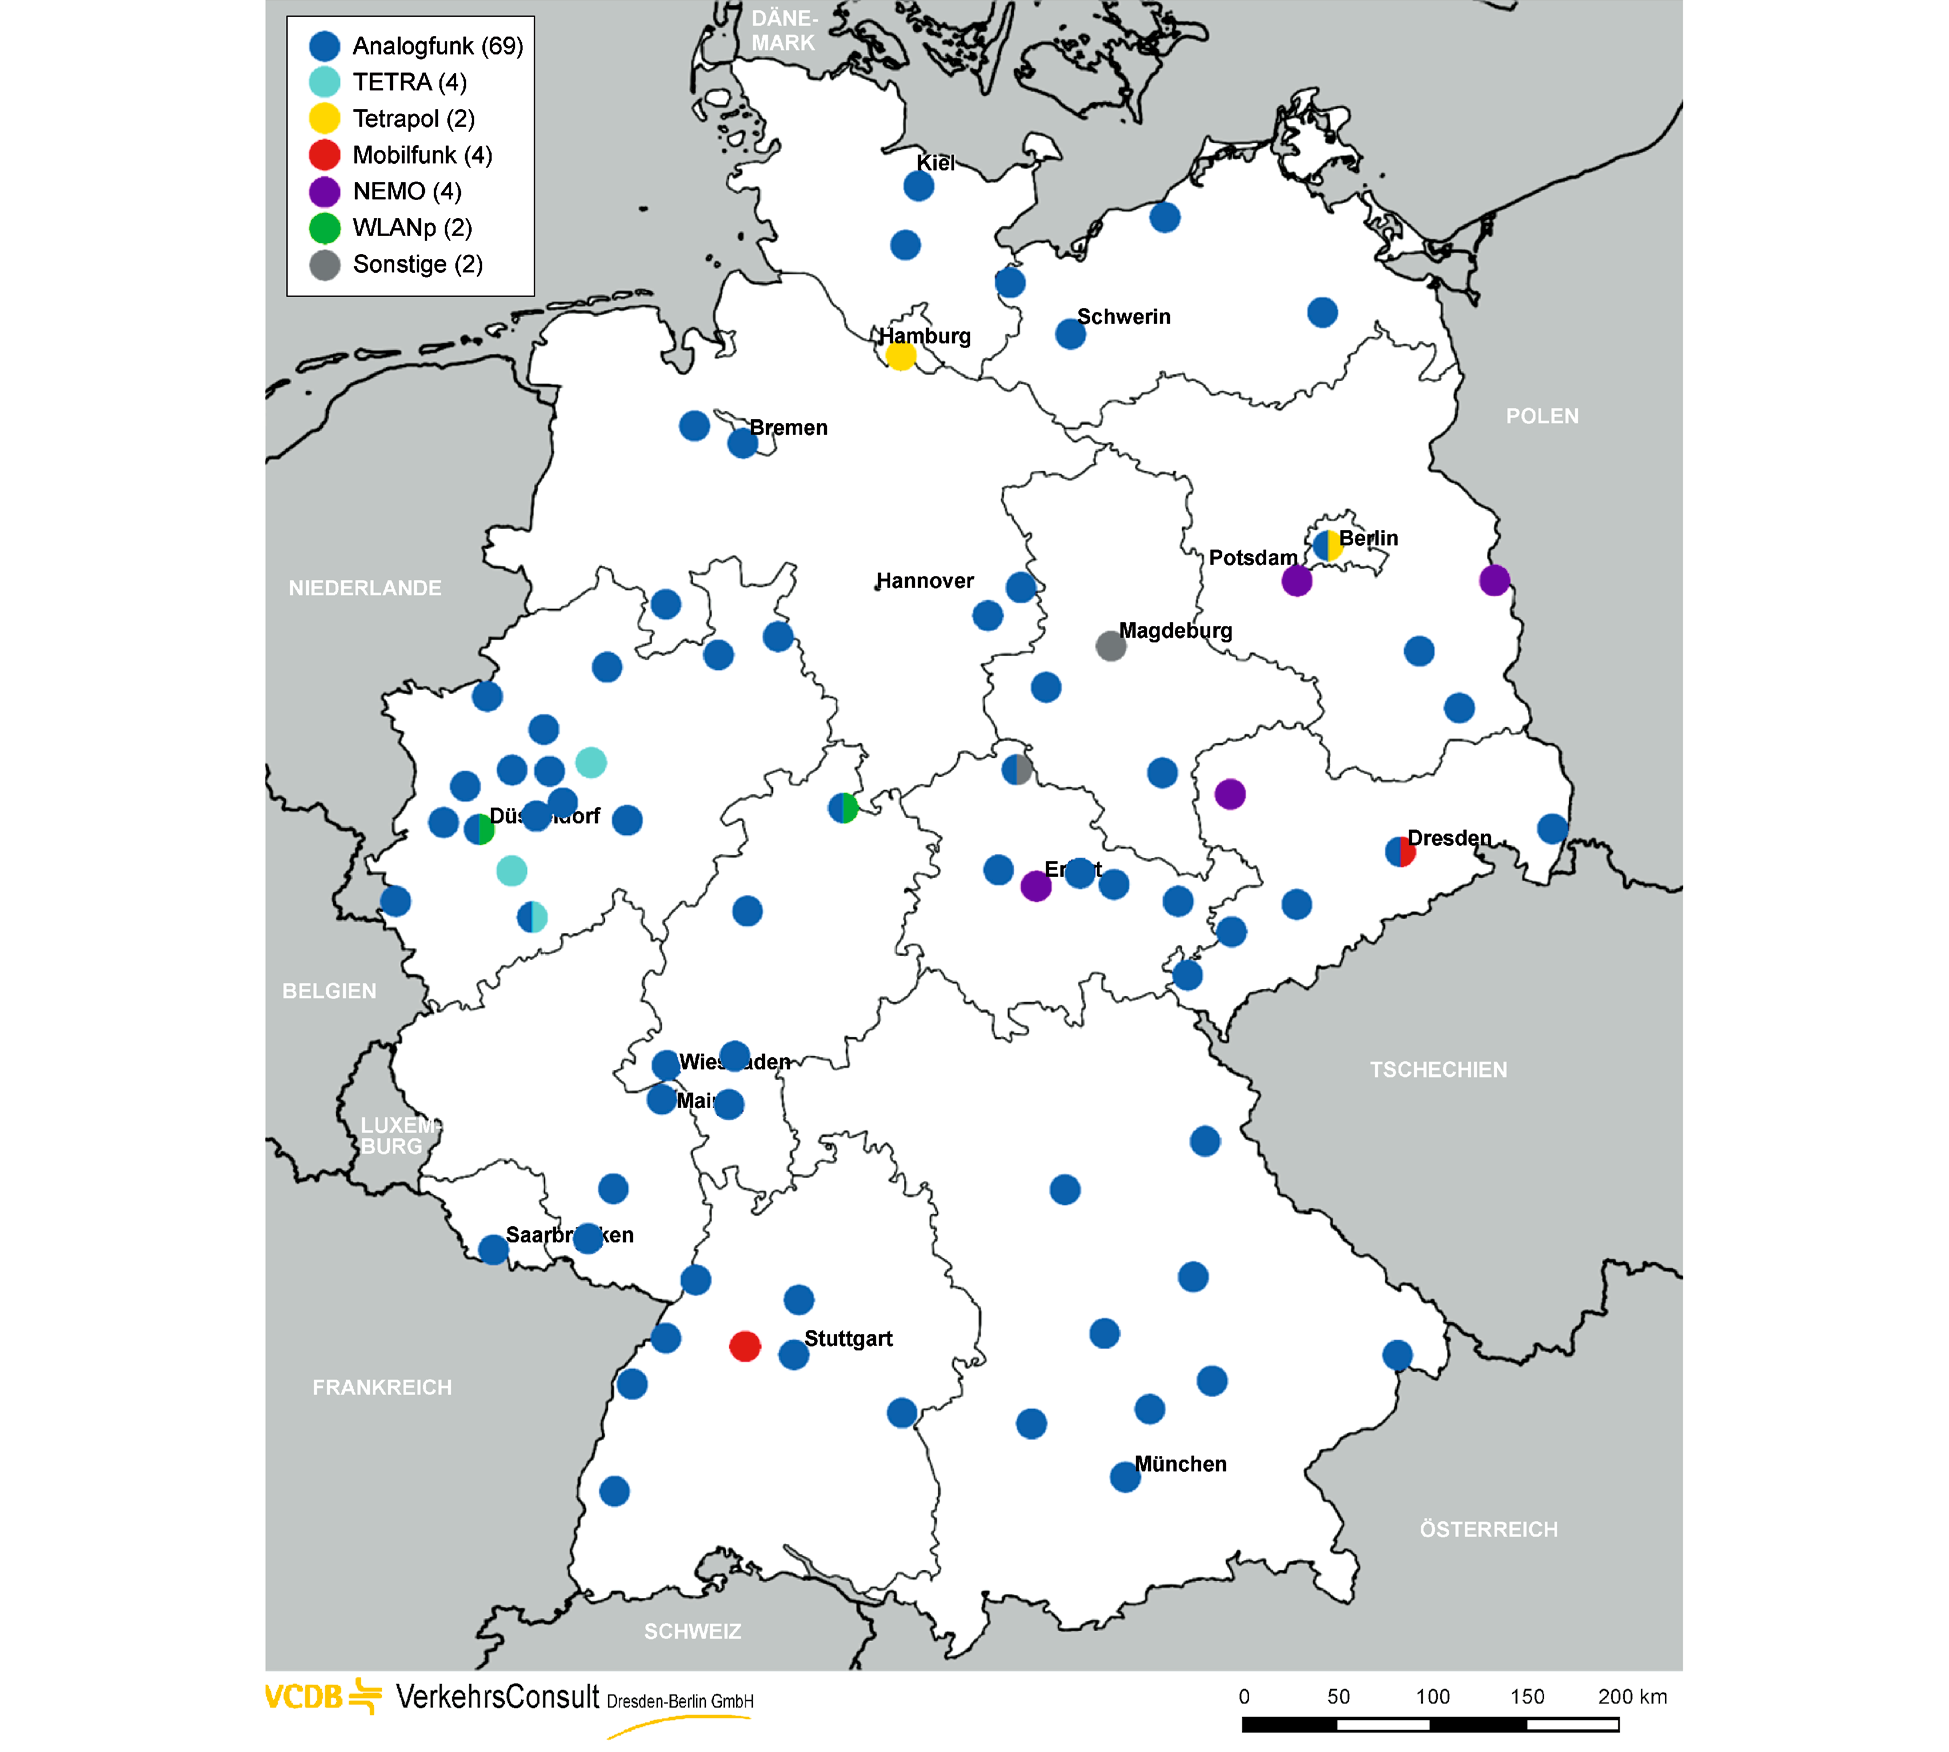
\includegraphics[height=0.8\textheight]{figs/vcdb-map-ampelbeeinflussung.png}
\end{frame}

\section{Soul Extrating Information \& Mapping }

%TODO: oxa

\section{Architecture \& Infra }

\end{document}
